\section {Дополнения}

  \begin{center}
  \large
  \bf Скремблирование и дескремблирование
\end{center}

{\bf {Скремблер}} (scramble — шифровать, перемешивать) — программное или аппаратное устройство (алгоритм), выполняющее скремблирование — обратимое преобразование цифрового потока без изменения скорости передачи с целью получения свойств случайной последовательности. После скремблирования появление «1» и «0» в выходной последовательности равновероятны. Скремблирование — обратимый процесс, то есть исходное сообщение можно восстановить, применив обратный алгоритм.

Применительно к телекоммуникационным системам скремблирование повышает надежность синхронизации устройств, подключенных к линии связи (обеспечивает надежное выделение тактовой частоты непосредственно из принимаемого сигнала), и уменьшает уровень помех, излучаемых на соседние линии многожильного кабеля. Другая область применения скремблеров — защита передаваемой информации от несанкционированного доступа.

Для алгоритмов скремблирования исключительно важны скорость работы и случайный характер последовательности, чтобы его нельзя было восстановить в случае несанкционированного перехвата. Процесс скремблирования может включать в себя добавление определенных компонент к исходному сигналу либо изменение важных частей сигнала для того, чтобы усложнить восстановление вида исходного сигнала либо для придания сигналу определенных свойств.

Скремблеры применяются в телефонных сетях общего пользования, спутниковой и радиорелейной связи, цифровом телевидении, а также для защиты лазерных дисков от копирования. Обычно скремблирование осуществляется на последнем этапе цифровой обработки непосредственно перед модуляцией.
Принцип скремблирования заключается в побитном изменении проходящего через систему потока данных. Основной операцией, используемой в скремблерах, является побитовый XOR.

Типы скремблеров:

 - Самосинхронизирующиеся скремблеры;
 
 - Аддитивные скремблеры (с установкой).
   
   \begin{center}
  \large
 \bf Самосинхронизирующиеся скремблеры
 \end{center}
 
Основной частью самосинхронизирующегося скремблера является генератор псевдослучайной последовательности (ПСП) в виде линейного n-каскадного регистра с обратными связями, как правило формирующий последовательность максимальной длины $2^n - 1$.

\subsubsection{Блок схема - Самосинхронизирующийся скремблер}
\begin{center}
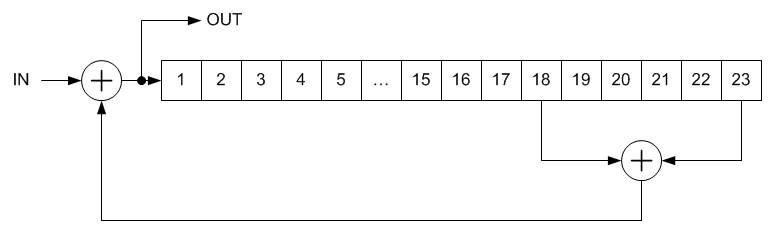
\includegraphics[scale = 0.6]{Scrambler_randomizer_multiplicative_scrambler}
 \end{center}
 
Особенностью самосинхронизирующегося скремблера является то, что он управляется скремблируемой последовательностью, то есть той, которая передаётся в канал. Поэтому при данном виде скремблирования не требуется специальной установки состояний скремблера и дескремблера: скремблированная последовательность записывается в регистры сдвига скремблера и дескремблера, устанавливая их в идентичное состояние. При потере синхронизма между скремблером и дескремблером время восстановления синхронизма не превышает числа тактов, равного числу ячеек регистра скремблера. 

На приёмной стороне выделение исходной последовательности происходит путём сложения по модулю 2 принятой скремблированной последовательности с последовательностью на выходе сдвигового регистра. Например, для схемы, приведенной на рисунке, входная последовательность IN с помощью скремблера в соответствии с соотношением $ OUT = IN+(R_{18}+R_{23})$ преобразуется в посылаемую двоичную последовательность OUT. В приёмнике из этой последовательности таким же регистром сдвига, как на приёме, формируется последовательность  $IN` = OUT + (R_{18}+R_{23}) = IN+(R_{18}+R_{23})+(R_{18}+R_{23}) = IN $.

Как следует из принципа действия схемы, при одной ошибке в последовательности IN ошибочными получаются также последующие восемнадцатый и двадцать третий символы (в данном примере). В общем случае влияние ошибочно принятого бита будет сказываться a раз, где a — число обратных связей в регистре сдвига. Таким образом, самосинхронизирующийся скремблер-дескремблер обладает свойством размножения ошибок. Данный недостаток самосинхронизирующегося скремблера- дескремблера ограничивает число обратных связей в регистре сдвига; практически это число не превышает $a = 2$.

Второй недостаток самосинхронизирующегося скремблера связан с возможностью появления на его выходе при определенных условиях так называемых «критических ситуаций», когда выходная последовательность приобретает периодический характер с периодом, меньшим длины ПСП. Чтобы предотвратить это, в скремблере и дескремблере предусматриваются специальные дополнительные схемы контроля, которые выявляют наличие периодичности элементов на входе и нарушают её.

   \begin{center}
  \large
 \bf Аддитивные скремблеры
 \end{center}
 
При аддитивном скремблировании требуется предварительная идентичная установка состояний регистров скремблера и дескремблера. В скремблере с установкой, как и в самосинхронизирующемся скремблере, производится суммирование входного сигнала и ПСП, но результирующий сигнал не поступает на вход регистра. В дескремблере скремблированный сигнал также не проходит через регистр сдвига, поэтому размножения ошибок не происходит.

\subsubsection{Блок схема - Аддитивный скремблер}
\begin{center}
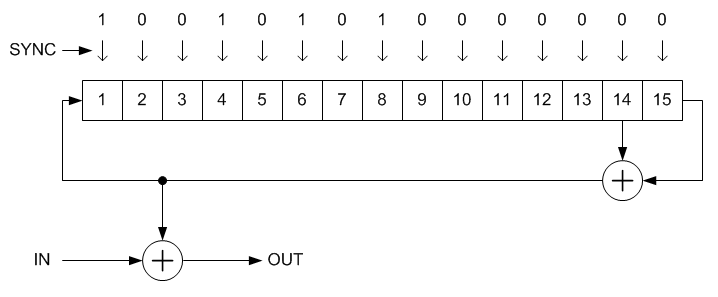
\includegraphics[scale = 0.6]{additive}
\end{center}

Суммируемые в скремблере последовательности независимы, поэтому их период всегда равен наименьшему общему кратному величин периодов входной последовательности и ПСП и критическое состояние отсутствует. Отсутствие эффекта размножения ошибок и необходимости в специальной логике защиты от нежелательных ситуаций делают способ аддитивного скремблирования предпочтительнее.

Реализация скремблера возможна как на электронной, так и на электрической базе, что и обеспечило его широкое применение. Факт, что каждый бит выходной последовательности зависит только от одного входного бита, также упрочил положение аддитивных скремблеров в защите данных. Это связано с неизбежно возникающими в канале передаче помехами, которые могут исказить в этом случае только те биты, на которые они приходятся.

Декодирование заскремблированных последовательностей происходит по той же самой схеме, что и кодирование.

Главная проблема аддитивных скремблеров — синхронизация передающего (кодирующего) и принимающего (декодирующего) устройств. При пропуске или ошибочном вставлении хотя бы одного бита вся передаваемая информация необратимо теряется. Поэтому, в системах на основе аддитивныъх скремблеров очень большое внимание уделяется методам синхронизации. На практике для этих целей обычно применяется комбинация двух методов: 

а) добавление в поток информации синхронизирующих битов, заранее известных приемной стороне, что позволяет ей при ненахождении такого бита активно начать поиск синхронизации с отправителем, 

б) использование высокоточных генераторов временных импульсов, что позволяет в моменты потери синхронизации производить декодирование принимаемых битов информации "по памяти" без синхронизации.

   \begin{center}
  \large
 \bf Регистр сдвига с линейной обратной связью
 \end{center}
 
Рассмотрим простой РСЛОС:
 
 Регистр сдвига состоит из  однобитовых ячеек $b_1$, $b_2$, . . . ,$b_n$ , содержащих 0 или 1, и линейной обратной связи. 
Начальным состоянием генератора является набор значений в битовых ячейках. На каждой итерации генератор вычисляет сумму по модулю два (то есть выполняет операцию XOR) значений ячеек.

\subsubsection{Блок схема - Регистр сдвига с линейной обратной связью}
\begin{center}
\includegraphics{{images}}
 \end{center}

Далее регистр сдвигает значения на одну ячейку влево. Самая правая ячейка $b_n$ принимает вычисленное значение $b_{n+1}$

Максимальный период последовательности РСЛОС равен $2^n - 1$. Максимум достигается в том и только в том случае, когда харак- теристический многочлен РСЛОС примитивен. В этом случае РСЛОС называют регистром сдвига максимального периода, а генерируемые им последовательности – М-последовательностями, или же последовательностями максимального периода.

Если известна структура РСЛОС, то внутреннее состояние генератора можно восстановить по  предыдущим выходам. По 2 предыдущим выходам генератора можно восстановить и внутреннее состояние, и структуру генератора. Зная структуру и текущее внутреннее состояние генератора, можно восстановить его предыдущие и следующие выходные значения.


   \begin{center}
  \large
 \bf Скремблирование для защиты телефонных переговоров и радиосвязи
 \end{center}

Скремблеры активно применяются для защиты телефонных и радио переговоров. При скремблировании возможно преобразование речевого сигнала по трем параметрам: амплитуде, частоте и времени. В системах подвижной радиосвязи практическое применение нашли в основном частотные и временные преобразования сигнала, а также их комбинации. Возможные помехи в радиоканале существенно затрудняют точное восстановление амплитуды речевого сигнала, в связи с чем амплитудные преобразования при скремблировании практически не применяются.

   \begin{center}
  \large
 \bf Динамические (роллинговые) скремблеры
 \end{center}

Все рассмотренные выше скремблеры предполагают фиксированные параметры преобразования сигнала (фиксированные ключи) в течение передачи речевого сообщения и поэтому называются статическими.
Дополнительное повышение уровня закрытия информации может быть обеспечено изменением параметров преобразования сигнала во времени. Такие скремблеры называются динамическими. В современной практике их часто обозначают термином роллинговые скремблеры.

Динамические скремблеры, как правило, существенно дороже скремблеров с фиксированными параметрами преобразования сигнала, сильнее влияют на характеристики радиосредств и требуют начальной синхронизации. Однако их применение действительно затрудняет возможности перехвата переговоров, в особенности в реальном масштабе времени. Это объясняется тем, что изменение ключевых параметров во времени теоретически делает возможным резкое увеличение количества ключей, под которыми для роллинговых скремблеров обычно понимают некоторое значение, определяющее порядок изменения параметров преобразования сигнала. Например, ключом может быть начальное значение генератора псевдослучайной последовательности, в соответствии с которой меняется определенный ключевой параметр.

Временные преобразования сигнала в сочетании с изменением ключевых параметров во времени сложны для реализации и требуют относительно длительной синхронизации, поэтому они пока не нашли свое применение в роллинговых скремблерах. Для способов частотного преобразования сигнала изменяемыми ключевыми параметрами могут быть частота инверсии (для частотного инвертора), частота разбиения полосы сигнала (для полосно-сдвигового инвертора), комбинация частотной перестановки поддиапазонов сигнала (для полосового скремблера). Большинство известных моделей роллинговых скремблеров используют наиболее простой принцип спектрального преобразования — частотный инвертор с изменением частоты инверсии сигнала во времени. Различие скремблеров состоит в числе частот инверсии, скорости их изменения и количестве ключей, определяющих длительность перебора возможных комбинаций изменяемых параметров без их повторения.






